%% Page settings.
\documentclass[10pt,a4paper,twoside]{article}
\usepackage[top=1.5in, left=1.2in, bottom=1.5in, right=1.2in]{geometry}
%==================================================%
%% Encoding packages.
\usepackage[UKenglish]{babel}
\usepackage[nodayofweek]{datetime}
\usepackage[T1]{fontenc}
\usepackage[utf8]{inputenc}
\usepackage{amsmath}
\usepackage{amsthm}
\usepackage{amsfonts}
\usepackage{amssymb}
\usepackage{calc}
\usepackage{natbib}
%\usepackage{grffile}
\usepackage{subcaption}
%==================================================%
%% Document details.
\usepackage{titling}
\title{Information and admissible sets}
\author{Jeff Rowley}
\newcommand{\thedate}{\today}
% Enter document details here.
\newcommand{\details}{C:/Dropbox/TeXTemplates/}
% Enter the file path here for the UCL logo and bibliography.
% Change this file path for different computer systems.
%==================================================%
%% Date macro.
\newcommand{\theseason}[1]{
\ifcase \month 
\or Winter\or Winter\or Spring\or Spring\or Spring\or Summer\or Summer\or Summer\or Autumn\or Autumn\or Autumn\or Winter\fi}
% Displays the season.
% Obsolete in this template.
%==================================================%
%% Useful packages.
\usepackage{enumerate}		% Lists.
\usepackage{bbm}			% Indicator functions.
\usepackage{lipsum}			% Random text generator.
\usepackage{MnSymbol}		% Arrows.
\usepackage{graphicx}		% Graphics.
%==================================================%
%% Theorem environments.
\newcounter{countthm}[section]
\newcounter{countlem}[section]
\newcounter{countex}[section]
% Creates new counters which reset at each new section. 
\renewcommand{\thecountthm}{\thesection.\arabic{countthm}}
\renewcommand{\thecountlem}{\thesection.\arabic{countlem}}
\renewcommand{\thecountex}{\thesection.\arabic{countex}}
% Redefines counters to include the section number.
\newtheorem{thm}[countthm]{Theorem}
% Creates a theorem environment - type \thm to begin.
\newtheorem{lem}[countlem]{Lemma}
% Creates a lemma environment - type \lem to begin.
\newtheorem{ex}[countex]{Example}
% Creates an example environment - type \ex to begin.
\newtheorem*{Acknowledgements}{Acknowledgements}
% Creates a thanks environment.
\newcommand{\newthm}[1]{\newtheorem*{#1}{#1}}
% A macro that makes defining new theorem environments quick.
% Type \newthm{<Theorem name here>} to begin.
%==================================================%
%% Math operators.
\DeclareMathOperator*{\plim}{plim}
% Writes plim in math environment - type \plim to enter.
\DeclareMathOperator*{\argmax}{argmax}
% Writes argmax in math environment - type \argmax to enter.
\DeclareMathOperator*{\argmin}{argmin}
% Writes argmin in math environment - type \argmin to enter.
\DeclareMathOperator*{\argsup}{argsup}
% Writes argsup in math environment - type \argsup to enter.
\DeclareMathOperator*{\arginf}{arginf}
% Writes arginf in math environment - type \arginf to enter.
\newcommand\independent{\protect\mathpalette{\protect\independenT}{\perp}} 
\def\independenT#1#2{\mathrel{\rlap{$#1#2$}\mkern2mu{#1#2}}} 
% Pastes an independence symbol - type \independent to enter.
%==================================================%
%% Equation numbering.
\numberwithin{equation}{subsection}
% Numbers equations up to the subsection. To change level,
% replace subsection with section.
%==================================================%
%% Counters.
\newcounter{saveenumi}
\newcounter{saveenumi1}
\setcounter{section}{0}
%==================================================%
\newcommand{\ESRC}{I acknowledge financial support from the Economic and Social Research Council (ESRC).}
%==================================================%
%% The title page.
\makeatletter				
% Changes @ to catcode 11.
\renewcommand{\@maketitle}{
\null
\graphicspath{ {\details} }
\flushleft{\includegraphics[width=40mm]{UCL_Logo_Orange}}
\hspace{5mm}
\normalsize Department of Economics, University College London\\
\vskip\bigskipamount
\leaders\vrule width \textwidth\vskip0.4pt 
\vskip\bigskipamount 
\nointerlineskip
% This completes the UCL banner.
\begin{center}
\begin{minipage}{100mm}
\begin{center}
\vspace{20mm}
\LARGE
\textbf{
\@title}
\par
\vspace{10mm}
\normalsize
\@author
\par
\vspace{5mm}
\normalsize
\thedate
\end{center}
\end{minipage}
\end{center}
}
\makeatother				
% Reverts @ to catcode 12.
%==================================================%
%% Packages to load at end of preamble. 
% Note conflict between Tkz-euclide package set and 
% game theory package set. Load one or the other.
\usepackage{hyperref}
%\usepackage[numbered]{mcode}

%% Tkz-euclide package set.
%\usepackage{tkz-euclide}
%\usepackage{pgfplots}
%\usepgfplotslibrary{external} 
%\tikzexternalize[prefix=tikz/]

%% Game theory package set.
\usepackage{pstricks}	
\usepackage{egameps}		 
\usepackage{pst-3d}			
\usepackage{sgame}	
\renewcommand{\gamestretch}{1.5}
%==================================================%
%% Further notes regarding egameps package.
% The egameps package is incompatible with this template
% due to UCL logo. Solution is to independently run 
% egameps through on a latex blank document, then insert 
% pdf into this document. Recall that to run egameps:
% "latex" --> "DVi->PS" --> "PS->PDF"
% then use "includegraphics[]" with trim option. 
%==================================================%
%% Headers and footers.
\usepackage{fancyhdr}
\pagestyle{fancy}
\renewcommand{\sectionmark}[1]{\markright{\thesection.\ #1}}
% This redefines the \rightmark command so that the section number does not appear.
% NOTE: To remove the section number, delete <<\thesection.\>>
\lhead[\thepage]{\rightmark}
\rhead[\rightmark]{\thepage}
\chead[]{}
\cfoot[]{}
\lfoot[\thetitle]{}
\rfoot[]{\theauthor}
\renewcommand*\thesection{\arabic{section}}
\usepackage{epigraph}
%==================================================%
%% Start of document.
\begin{document}
\maketitle
\vspace{10mm}
\begin{abstract}
\noindent <<Abstract here>>
\begin{Acknowledgements}
<<Acknowledgements here>>
\ESRC
\end{Acknowledgements}
\end{abstract}
\vspace{5mm}
%==================================================%
%% Document.
%==================================================%
\section*{Notation}
There is a probability space $(\Omega,\Sigma,\mathbb{P})$ on which are defined random variables $(Y,D,X,Z,U)$. Here, $(Y,D,X,Z)$ are observable with supports $(\mathcal{R}_Y,\mathcal{R}_D,\mathcal{R}_X,\mathcal{R}_Z)$, and $U$ is unobservable with as yet unspecified support. I allow $(X,Z,U)$ to be vectors, in which case the support is given by the Cartesian product of the supports of each element in the vector. I refer to $Y$ as the dependent variable, to $D$ as the endogenous variable, to $X$ as the exogenous variable, to $Z$ as the instrumental variable, and to $U$ as unobservable heterogeneity. The logic of this naming convention will be made clear by the restrictions that are imposed upon these random variables in the main text. Lower case letters are used to represent specific values of these random variables.

I denote by $Y(d)$ the counterfactual value of $Y$ when $D$ is externally fixed, and by $D(z)$ the counterfactual value of $D$ when $Z$ is externally fixed. I denote by $\mathbb{E}$ the expectation operator, and  by $\mathbbm{1}$ the indicator function. Related to these concepts are the average causal effects $ACE(D\rightarrow Y)$ and $ACE(Z\rightarrow D)$ that are defined as $\mathbb{E}[Y(d_1)-Y(d_0)]$ and $\mathbb{E}[D(z_1)-D(z_0)]$ when $(D,Z)$, respectively. To distinguish between population and sample quantities, I subscript sample quantities by $n$. 
%==================================================%
\section{Introduction}
I explore the effect of incorporating information on the identified set of values for a non-parametric model that permits non-random selection by agents into treatment groups, and that embeds an exclusion restriction and an independence restriction that characterise an instrumental variable. I consider the effect of combining many instrumental variables into a composite instrumental variable with many points of support on the identified set of values for counterfactual outcome distributions. Further, I consider the effect of enriching individual behaviour by allowing relevant exogenous variables to affect individual choice over treatment and outcomes. I establish the conditions under which the parameter of interest in the enriched model is equivalent to the parameter of interest in a model that does not explicitly account for the contribution of additional relevant exogenous variables beyond the endogenous variable of interest.

The model that I consider is partially identifying. That is, the restrictions on the set of admissible structures (or data generating processes) that are implied by the model are insufficient to exclude observationally equivalent structures; an identifying correspondence from a probability distribution to the set of structures that are admitted by the model is a one-to-many function. 
%==================================================%
\section{A threshold crossing model}
I 
%==================================================%
%% Diagrams
\begin{figure}[p]
\centering
\begin{subfigure}{0.8\textwidth}
  \centering
  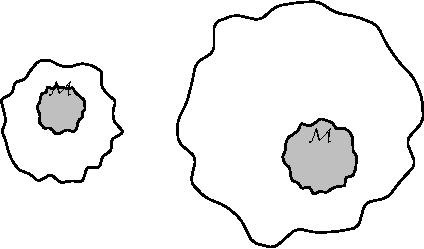
\includegraphics[width=\textwidth]{C:/Users/Jeffro/Documents/GitHub/Covariatesets/Diagrams/Identification.pdf}
  \caption{A model $\mathcal{M}$ is a set of structures that forms a proper subset of the class of all structures $\mathcal{S}$. Each structure in $\mathcal{M}$ generates a probability distribution in the class of all probability distributions (of observable variables) $\mathcal{P}$, the union of which is the image set $\mathcal{I}$. Then $\mathcal{I}$ is the set of all probability distributions that are generated by $\mathcal{M}$.}
  \label{fig:sub1}
  \end{subfigure}
\begin{subfigure}{0.8\textwidth}
  \centering
  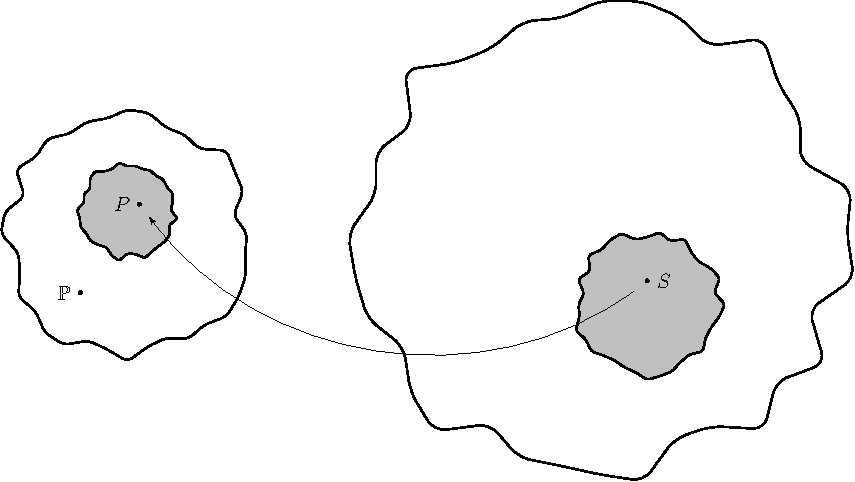
\includegraphics[width=\textwidth]{C:/Users/Jeffro/Documents/GitHub/Covariatesets/Diagrams/Observationalrestrictiveness.pdf}
  \caption{A structure $S$ is said to be observationally restrictive if it generates a probability distribution $P$ such that $P\in\mathcal{P}\setminus\mathcal{I}$. If all $S\in\mathcal{M}$ are observationally restrictive then $\mathcal{M}$ is observationally restrictive, and is falsified.}
  \label{fig:sub2}
  \end{subfigure}
\caption{Structures, models, probability distributions (of observable variables), and falsifiability.}
\label{fig:test1}
\end{figure}
\begin{figure}[p]
\centering
\begin{subfigure}{0.8\textwidth}
  \centering
  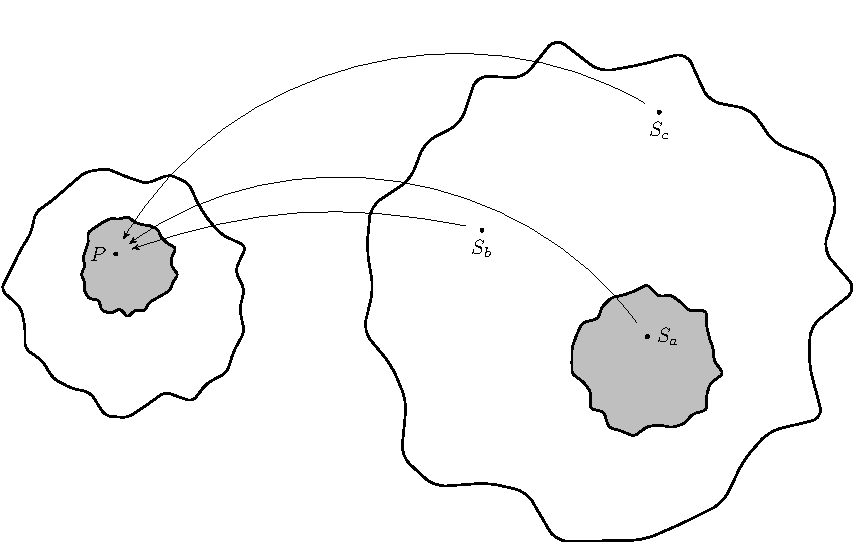
\includegraphics[width=\textwidth]{C:/Users/Jeffro/Documents/GitHub/Covariatesets/Diagrams/Pointidentification.pdf}
  \caption{A model $\mathcal{M}$ is said to identify a structure $S$ if the probability distribution (of observable variables) $P$ that is generated by $S$ is distinct from those generated by other structures in $\mathcal{M}$. The structures $S_a$, $S_b$ and $S_c$ are said to be observationally restrictive as they all generate $P$ but $S_b$ and $S_c$ are not admitted by $\mathcal{M}$. As $S_a$ is the only structure that is admitted by $\mathcal{M}$ and that generates $P$, $S_a$ is identified by $\mathcal{M}$. For completeness, $\mathcal{M}$ is said to be uniformly identifying if it identifies each structure that it admits.}
  \label{fig:sub3}
  \end{subfigure}
  \begin{subfigure}{0.8\textwidth}
  \centering
  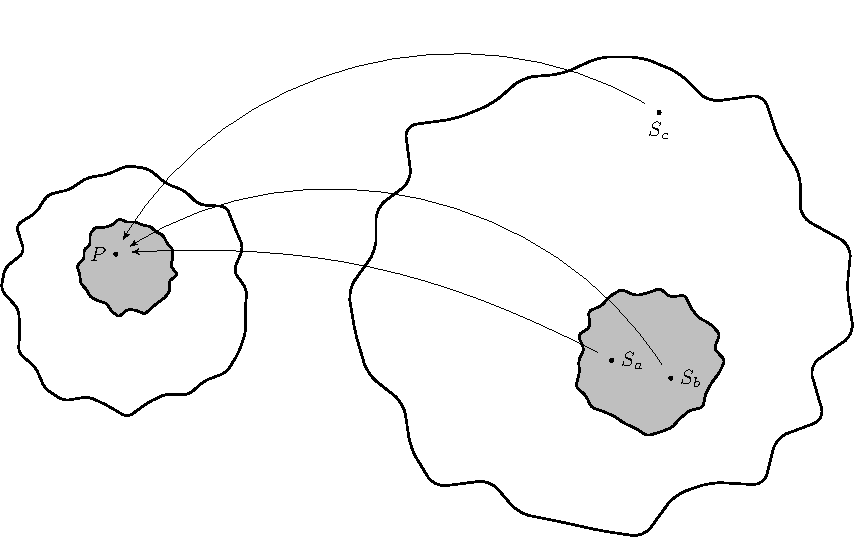
\includegraphics[width=\textwidth]{C:/Users/Jeffro/Documents/GitHub/Covariatesets/Diagrams/Setidentification.pdf}
  \caption{As $S_a$ and $S_b$ are observationally equivalent and are both admitted by $\mathcal{M}$ then $\mathcal{M}$ does not identify either $S_a$ or $S_b$. Nonetheless, as $\mathcal{M}$ restricts the set of observationally equivalent structures that generate $P$ to $S_a$ and $S_b$ then $\mathcal{M}$ partially identifies $S_a$ (and $S_b$ to within $\lbrace S_a,S_b\rbrace$).}
  \label{fig:sub4}
  \end{subfigure}
\caption{Identification and non-identification of a structure, and partial identification of a structure.}
\label{fig:test}
\end{figure}
%==================================================%
%% Bibliography.
\bibliographystyle{chicago}
\bibliography{\details Bibliography}
\end{document}
